\section{径向记录道}
\label{sec:5.1}

作为共炮检距剖面的一个变种,
在\ref{sec:3.6}节内曾介绍过径向记录道剖面,\ref{sec:3.6}节的目的是要使非零炮检距资料达到适当的偏
移。我们也理解了倾角时差校正(DMO)的定义,DMO使问题的深入分析得到简化,
因为在倾角时差校正之后我们可以分析假想的由水平分层地层所产生的道集。

径向记录道道集定义为普通道集的一种变形。设普通道集记为$P(x,t)$,令径向参
量记为$r=x/t$,于是径向记录道道集$P'(r,t)$就按变形定义为$P'(r,t)=P(rt,t)$。

射线尖端的水平位置x按照关系$x=vt\sin\theta$而移动,所以在某种恒定速度介质中,具有
固定关系$r=x/t$的径向记录道包含有所有以角度$\theta$而传播的能量。

在一个径向记录道之内的传播角度恒定应有助于对多次反射的分析。由于爆炸与检波器
组合的方向特性对每个径向记录道都是时不变的(time-invariant),这种角度恒定性也将有
助于对爆炸波形进行补偿。

设反射面位于深度$z_j$且速度为常数,各双曲线形时距曲线为
\begin{equation}
t^2v^2=x^2+z^2
\label{eq:ex5.1.1}
\end{equation}
让我们看一下,当炮检距x变换成径向参量$r=x/t$
时,双曲线会出现什么变化。我们得到图\ref{fig:slnt/fronts}显示$(r,t)$平面内一个曲线族的方程为
\begin{equation}
z_j^2=t^2(v^2-r^2)
\label{eq:ex5.1.2}
\end{equation}

渐近线不再是沿着倾斜直线$x^2=\pm v^2t^2$
分布,而都是沿垂直线$r=\pm v$分布。$(r,t)$
平面被填满的区域呈矩形,而$(x,t)$平面被填满的区域则呈三角形。

图\ref{fig:slnt/radial2}所示为变换至径向空间之前与之后的野外剖面.在各个真正的记录道之间混杂
有零记录道,以便使变形的形状能够清晰显示;记住野外记录道是常数值情形下的一条
曲线,将有助于理解认识这种变形。

径向记录道变换的一个有趣方面是它对地滚波的影响问题。以某种恒定速度沿水平方向
传播的波就是地滚波的一种筒单模型,所以,在径向记录道道集中可以发现地滚波犹如是在
$r=\pm v_{roll}$附近少数径向记录道中的直流成分(零频率)。图\ref{fig:slnt/radial3}所示是一种近似于理想
化的情形。

\begin{figure}[H]
\centering
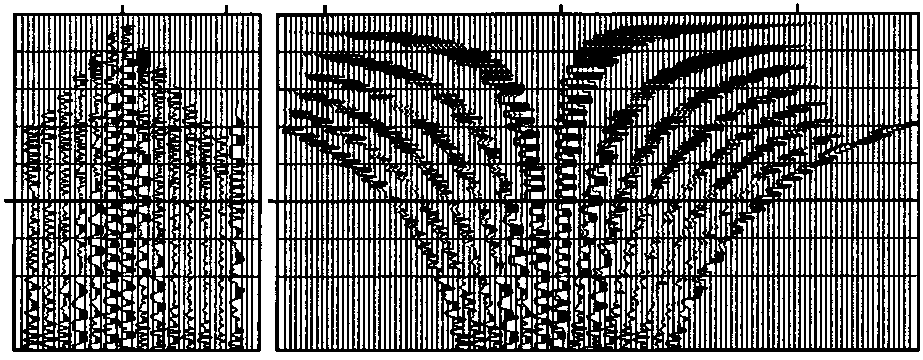
\includegraphics[width=0.65\textwidth]{slnt/radial2}
\caption[radial2]{混杂有零记录道的Alberta地区野外剖面(西方地球物理公司提供)。
所示为径向记录道变形之前(左图)和之后(右图)的面貌}
\label{fig:slnt/radial2}
\end{figure}

\begin{figure}[H]
\centering
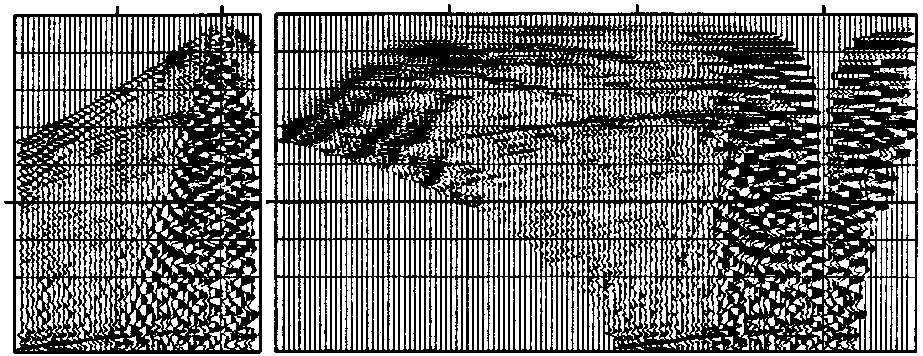
\includegraphics[width=0.65\textwidth]{slnt/radial3}
\caption[radial3]{Alberta地区野外剖面(西方地球物理公司提供)。
所示为变形为径向记录道之前(左图)和之后(右图)的情形}
\label{fig:slnt/radial3}
\end{figure}

\subsection{时差校正径向记录道}
\label{sec:5.1.1}

时差校正可以看成是一种从时间到深度的变换,在适当地完成了时差校正时,所有记录
道都应表示相同的与深度有关之反射率(reflectivity
),在原理上,径向时差校正是以引入z并利用代换$tv=\sqrt{z^2+x^2}$消去t的办法进行的;
在实际作时,你会更喜欢采用从旅行
时间深度坐标变换至深度坐标的办法。因此变换方程变为
$t=\sqrt{r+x^2/v^2}$,利用rt消去x,我们得到
\begin{equation}
t=\frac{r}{\sqrt{1-r^2/v^2}}
\label{eq:ex5.1.3}
\end{equation}

检查一下式\ref{eq:ex5.1.3}我们就会明白,径向记录道坐标中的时差校正就是时间t坐标轴均
匀压缩成r坐标轴。在r固定时,压缩量是固定的,压缩量并不随时间而变化。压缩的均匀性有助
于模拟和消除爆炸波形与多次反射的影响。要注意奇妙的是:径向记录道的时差校正是压缩
时间,而共炮检距资料的时差校正却是均匀地拉伸时间。图\ref{fig:slnt/radial3}
所示是径向记录道变换之前与之后的野外剖面。

\subsection{Snell记录道}
\label{sec:5.1.2}

不论地层速度如何,均可采用径向记录道坐标系统,但是在速度为常数时该坐标系统却有
特殊的好处,因为这时它采集的是某一固定传播角度的所有能量;合乎逻辑地推广至分层介质
时,则必然是采集具有某一固定Snell参量的所有能量。Snell记录道定义为$(x,t)$平面上的这
样一种轨迹:如速度为$v(z)$,该轨迹处处满足时差$p=dt/dx$为常数(据Ottolini的定义)。
在速度随深度而增大之处,该Snell记录道弯曲向上。对射线方程进行积分,很容易求出
Snell记录道轨迹为
\begin{subequations}
\begin{equation}
x=\int_0^z\tan\theta dz
\label{eq:ex5.1.4a}
\end{equation}
\begin{equation}
t=\int_0^z \frac{dz}{v\cos\theta}
\label{eq:ex5.1.4b}
\end{equation}
\label{eq:ex5.1.4}
\end{subequations}

为对Snell记录道进行时差校正,引入垂直旅行时间深度$\tau$,使得$dz=vd\tau$,于是径向记
录道的时差校正方程成为:
\begin{subequations}
\begin{equation}
x(p,\tau)=\int_0^\tau \frac{pv^2}{\sqrt{1-p^2v^2}}d\tau
\label{eq:ex5.1.5a}
\end{equation}
\begin{equation}
t(p,\tau)=\int_0^\tau \frac{1}{1-p^2v^2}d\tau
\label{eq:ex5.1.5b}
\end{equation}
\label{eq:ex5.1.5}
\end{subequations}

在地层速度为分层速度之处,Snell记录道具有胜过径向记录道的某种理论优点。可是它
们也有不利之处:曲线可能变成了多枝的,以致变换将不再一一对应。所以,在实际应用
时,你也许要用一个简化速度模型来代替你对真速度的最佳估计才行。

用更富哲理的譬喻来说,从共炮检距记录道过渡至径向记录道是个千元钞票(big
one),而从径向记录道过渡至Snell记录道则不是如此大面额。由于径向记录道还未广泛采
用,我们可以推测Snell记录道的实用性可能要受到进一步的限制。



